\chapter{Глава про симуляцию: с картинками и табличками}
\label{cha:simulation}
\thispagestyle{chapterpage}

Вообще-то подобная нумерация не характерна для книг, но поведение параграфов соответствует пунктам и подпунктам отчета.

\section{Обобщенная модель навигационного сигнала ГНСС}

\paragraph{}В разделе тоже могут быть пункты

\paragraph{}И ещё

\subparagraph{}И подпункты

\paragraph{}Обратите внимание, что нумерация пунктов согласована с их положением в иерархии разделов


\subsection{Модель традиционного BPSK сигнала}

\paragraph{}И в подразделе могут быть пункты!

\paragraph{}И ещё

\subparagraph{}И подпункты

\paragraph{}Обратите внимание, что нумерация пунктов согласована с их положением в иерархии разделов

Обратимся к опыту спутниковых навигационных систем. 
Они развиваются уже более полувека, пройдя через множество модификаций и смену поколений. 
Эволюция этих систем сопровождалась развитием используемых сигналов: от простых двухтоновых колебаний до многокомпонентых сигналов с криптографической защитой. 

\begin{figure}[ht]
  \centering
  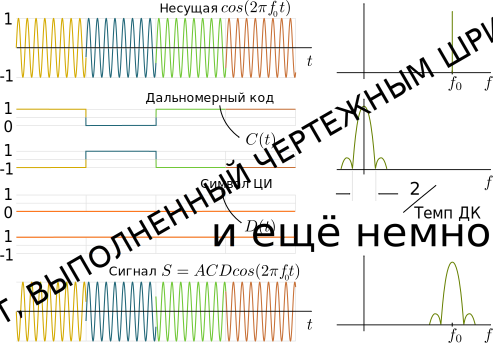
\includegraphics[keepaspectratio, width=0.8\textwidth]{inc/svg/simulation/LegacySignalsOscSpectr}
  \caption{Структура сигнала ГНСС с модуляцией дальномерным кодом и навигационным сообщением}
  \label{fig:LegacySignalsOscSpectr}
\end{figure}

В широко используемых сигналах GPS L1C/A и ГЛОНАСС L1OF в качестве спектрорасширяющей последовательности используются дальномерные коды с периодом в 1 мс и длиной 1023 и 511 символов соответственно. 
Эти последовательности являются псевдослучайными (ПСП, англ. PRN), формируются с помощью линейных генераторов на сдвиговых регистрах (англ. LFSR). 
Модель таких сигналов проста (см. рис.~\ref{fig:LegacySignalsOscSpectr}):
\begin{equation}
S\left( t  \right) = A C D \cos \left( 2 \pi f_0  t  + \varphi \right),
\end{equation}
где
\begin{itemize}
\item $A$ -- амплитуда сигнала, больше или равна нулю;
\item $C = C\left( t  \right)$ -- модуляция дальномерным кодом, принимает значения $+1$ и $-1$ при значениях дальномерного кода $0$ и $1$ соответственно, смена значений происходит часто (2 мкс или менее);
\item $D = D\left( t \right)$ -- модуляция цифровой информацией, принимает значения $+1$ и $-1$ при значениях символа цифровой информации $0$ и $1$ соответственно, смена значений происходит редко (2 мс или более);
\item $f_0$ -- несущая частота, например, 1575.42 МГц для GPS L1C/A.
\end{itemize}

\begin{figure}[ht]
  \centering
  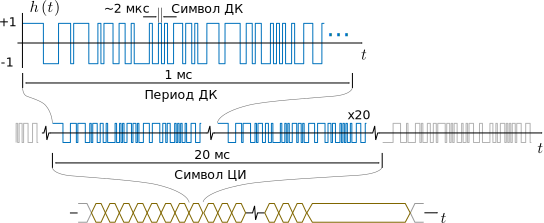
\includegraphics[keepaspectratio, width=0.8\textwidth]{inc/svg/analysis/hgraph0}
  \caption{Соотношение между темпом дальномерного кода и цифровой информации на примере сигнала ГЛОНАСС L1OF}
  \label{fig:hgraph0}
\end{figure}

Например, для всех сигналов ГЛОНАСС L1OF, принимаемых большинством современных смартфонов, используется один и тот же дальномерный код, повторяющийся каждую \textbf{миллисекунду} из года в год (см. рис.~\ref{fig:hgraph0}).

Ссылка, что уже встречалась в другой главе \autocite{basile2018}. 
А этой не было \cite{babyrov2013}

{
\renewcommand*{\bibfont}{\small}
\printbibliography[heading=subbibforcha, segment=\therefsegment]
}
